\chapter{Implementation of the Trading Systems}
This section provides a comprehensive overview of the two trading system implementations. The first focuses on the backtesting system, which simulates and evaluates strategies in a controlled environment. In this system, historical market data is utilised to test and analyse the performance of various strategies. The second implementation is the live system, designed to execute trades on the Ethereum blockchain using smart contracts. This system operates in real time and interacts with the live market, allowing actual trades to be executed based on predefined strategies. Together, these two implementations provide a comprehensive framework for testing, evaluating, and deploying trading strategies in simulated environments and on the live blockchain.

\section{Backtesting System}
\label{sec:backtesting-sys}

To develop a resilient backtesting system, a dedicated class was constructed to streamline the process of testing trading strategies; the system is entirely written in Python as it possesses countless libraries, including Pandas and Numpy, which are extensively used for data manipulation and analysis, it also is good with integrating with many data sources such as GraphQL which is required for this project. To evaluate a particular strategy, the \texttt{backtest} function requires \texttt{cointegrated\_pair}, a tuple of the names of the liquidity pools that the strategy is to be evaluated on, \texttt{strategy}, the strategy, and finally, the \texttt{initial\_investment} in ETH. The first argument is required and used to retrieve the relevant historical prices. The second parameter is self-explanatory, the strategy to test. Finally, including the initial investment amount as an input parameter enables users to simulate the performance of their strategies with a specific starting capital; it also helps analyse how the various transaction costs affect the ability to trade if any trades result in a loss. The \texttt{backtest} function iterates through historical data calling the strategy's \texttt{generate\_signal} and executing the trade orders it receives at each timestep. However, historical data is required; hence, the first step is to collect the historical data. The logical process of backtesting a pair can be seen in Figure \ref{fig:backtesting-flow}.
\begin{figure}[H]
    \centering
    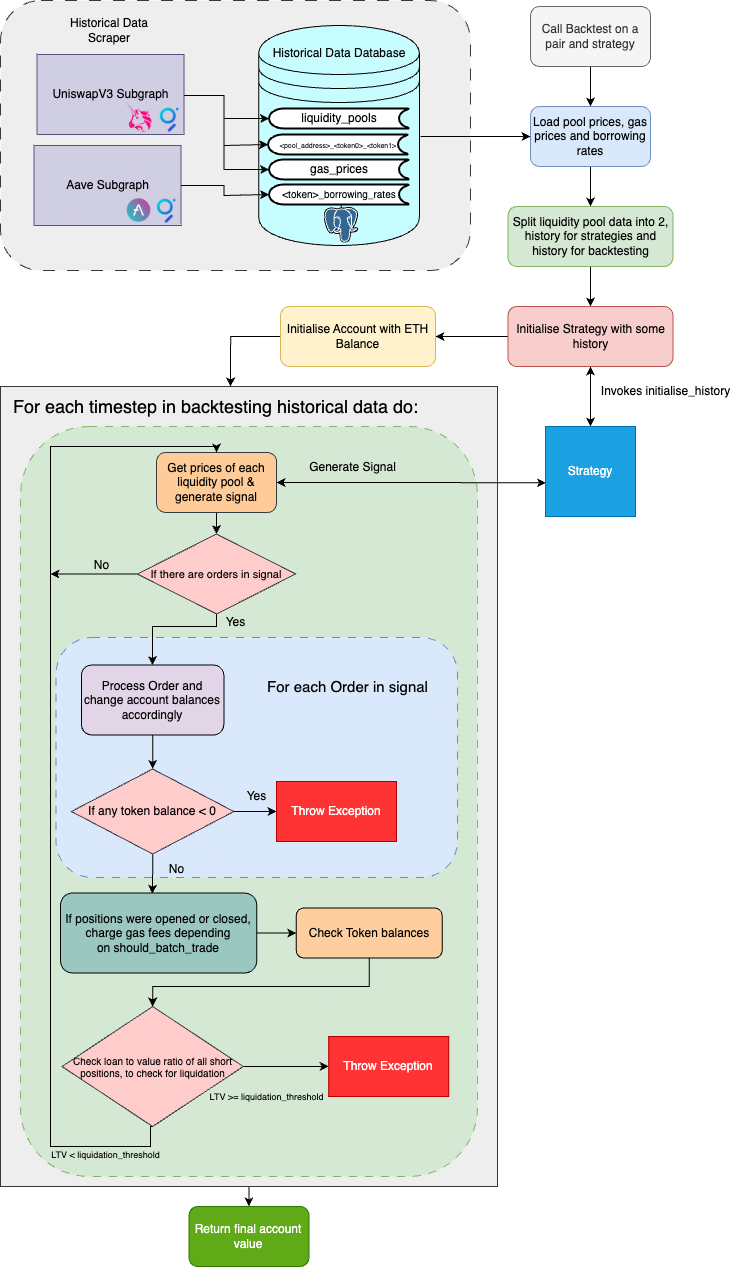
\includegraphics[width=0.99\textwidth]{project/Images/backtesting-diagram.png}
    \caption{Flowchart of backtesting a strategy on a liquidity pool pair \label{fig:backtesting-flow}}
\end{figure}

\subsection{Data Collection and Storage}
In order to simulate the market as accurately as possible, the system should have access to reliable and accurate historical market data, including price, volume, and other relevant indicators. Therefore, all of the data is retrieved from the Uniswap and Aave protocols' subgraph using the Graph~\cite{noauthor_graph_nodate}. The Graph is a decentralised protocol for indexing and querying blockchain data, making the data provided 100\% reliable as it indexes directly on the Ethereum blockchain. Subgraphs are GraphQL APIs designed to facilitate querying and extracting data from the blockchain. These APIs adhere to a specific schema outlined by the protocol, enabling seamless communication between the protocol and the underlying blockchain. Therefore, the Uniswap V3, Aave V2, and Aave V3 subgraphs are used to obtain the data required for the backtesting system.
\\[3mm]
In order to store the necessary data for backtesting and trading, a PostgreSQL database is used to provide consistency and flexibility, supporting numerous data types and a large set of SQL functions that allow for advanced querying. The database adopts the following schema:
\begin{figure}[!htb]
    \centering
    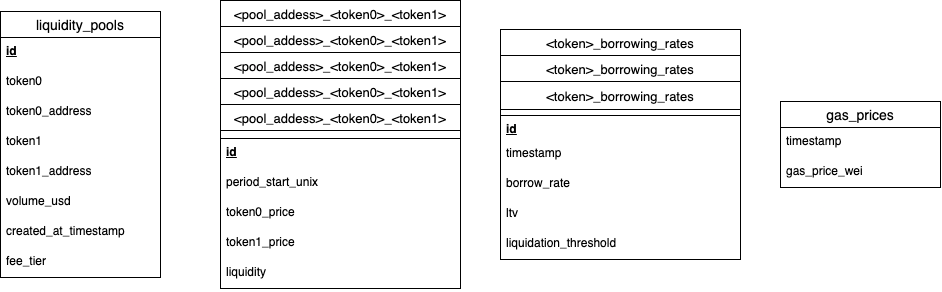
\includegraphics[width=0.8\textwidth]{project/Images/database_tables.png}
    \caption{Tables contained in the database \label{fig:database}}
\end{figure}
\\[3mm]
The \texttt{liquidity\_pools} contains data about the liquidity pools on Uniswap V3. After obtaining all of the data, it is found that it possesses 12,182 liquidity pools. However, most of these pools exhibit minimal or negligible trading volume. As a result, a criterion is established to selectively include only those liquidity pools that involve tokens supported by Aave and possess a trading volume exceeding \$10,000,000 (or \$10 million). This filtering condition ensures that the collected and stored data holds significance and relevance for research purposes, as these pools would allow for short selling.
\\[3mm]
Once these pools have been identified, pricing data about each pool that meets this condition is collected again using the Uniswap V3 subgraph. The query returns an array of dictionaries containing the pre-specified pricing data points at a frequency of every hour. Due to the limitations imposed by the subgraph, the results are constrained to a maximum size of 1000 entries. Hence, the query is executed iteratively to overcome this limitation and obtain the complete dataset. The previous maximum time, referred to as \texttt{prev\_max\_time}, is passed as an argument in subsequent queries to fetch the remaining data, i.e. \texttt{prev\_max\_time = hourlyData[-1]['periodStartUnix'] if len(hourlyData) > 0 else prev\_max\_time}. This data is stored in tables of the form \textit{<pool\_address>}\_\textit{<token0>}\_\textit{<token1>}.
\\[3mm]
Similarly, obtaining the interest rates for borrowing necessitates the utilisation of two of Aave's subgraphs. This requirement arises due to Aave's migration to Version 3 in March 2022, resulting in a transitional period where Uniswap V3 and Aave V2 were concurrently utilised. The schemas for the two are different; however, for the data we require, the borrowing rate, loan-to-value and liquidity threshold, the schema is consistent, and the same query can be used; this can be seen in Appendix \ref{app:lending-query}. During the table initialisation process, requests are made to the V2 and V3 GraphQL endpoints. However, only the V3 endpoint is utilised for sending requests when updating the table. The data is stored in tables of the form \textit{<symbol>}\_borrowing\_rates, where \textit{<symbol>} are all of the tokens that are present in the liquidity pools that are of interest.
\\[3mm]
The transaction history is queried at each hour to collect the gas price history since Uniswap migrated to V3. This is because querying in the same as the pricing data and borrowing rate history is too exhaustive as transactions occur every second. Therefore, it is more efficient to query at each hour with a window to retrieve the gas price at the closest hour as follows. Algorithm \ref{alg_gas_price_col} in the Appendix shows the pseudocode gas price at each hour is queried. 
\subsection{Types of Orders and Execution}
There are numerous order types that the backtesting supports due to measures to ensure a positive balance and avoid liquidation. The types of orders are; \texttt{BUY\ ETH}, \texttt{WITHDRAW}, \texttt{DEPOSIT}, \texttt{SWAP}, \texttt{OPEN\ BUY}, \texttt{CLOSE\ BUY}, \texttt{OPEN\ SELL}, \texttt{CLOSE\ SELL}. The procedures of the execution each order type are outlined below. The code of the execution, excluding gas fees, of the order is outlined in Appendix \ref{sec:backtesting-execution-code}.
\vspace{-3mm}
\paragraph{\texttt{BUY\ ETH}}
The \texttt{BUY\ ETH} order is used to swap a percentage of the accounts balance of WETH to ETH. The argument is a float between 0 and 1.
\vspace{-3mm}
\paragraph{\texttt{SWAP}}
The \texttt{SWAP} order is to execute a simple swap for either token0 or token1 of the liquidity pool. This order is only used as a precautionary order if the balance of the WETH balance gets too low. It takes two arguments, the first indicating whether it is swapping for token0 or token1, and the second parameter is a list of swaps, tuples containing with pool and the quantity that would like to be swapped. The amount received in the account is multiplied by \texttt{(1 - swap\_fees[swap\_token])}, this is because Uniswap charges a percentage of the swap specified by \texttt{swap\_fees[swap\_token]}.
\vspace{-3mm}
\paragraph{\texttt{OPEN\ BUY}}
Similar to the \texttt{SWAP} order, \texttt{OPEN\ BUY} opens a buy position. As mentioned above, opening a buy order is simply swapping token1 for token0. The parameters of buying are the target token and the volume. 
\vspace{-3mm}
\paragraph{\texttt{CLOSE\ BUY}}
Closing a buy position is similar to opening a buy position; however, the swap is in the other direction, i.e. from token to WETH. The only argument is the id of the buy order. To account for Uniswap's fees, the volume received after the initial swap is calculated and then swapped back to WETH.
\vspace{-3mm}
\paragraph{\texttt{OPEN\ SELL}}
Opening a sell position involves borrowing a token and then swapping the token. The parameters of selling are the target token and the volume. It also consists of depositing the required amount to borrow the volume ordered, calculated by the value-to-loan ratio.
\vspace{-3mm}
\paragraph{\texttt{CLOSE\ SELL}}
Closing a sell position is more complicated; it requires swapping back from the token to WETH, repaying the loan with interest and finally returning collateral. Swapping back to the required amount of tokens is the first step. For this, the variable Annual Yield Rates between the timestamp of the opening and the closing position are used to calculate the amount of interest required to be paid, as this is cumulated every second. Once the volume of tokens required to be returned is calculated, the equivalent amount of WETH plus accounting for Uniswap fees is swapped to obtain these tokens. Finally, the tokens are repaid, and the collateral is returned.
\vspace{-3mm}
\paragraph{\texttt{WITHDRAW}}
The \texttt{WITHDRAW} order's function is to withdraw some collateral stored in Aave. It is not used in the strategies however is implemented in case of developing further strategies that may require this functionality. The only parameter is the amount that would like to be withdrawn.
\vspace{-3mm}
\paragraph{\texttt{DEPOSIT}}
The \texttt{DEPOSIT} order's function is to deposit some additional collateral stored in Aave. This order is used when the collateral value not properly covering the loan value, hence avoiding liquidation. The only parameter is the amount that would like to be deposited. 

\subsection{Gas Fees}
To best approximate the gas fee, it is paramount to have an approximation of how much gas is used in each. Therefore, the smart contract for trading was written and run on a forked Ethereum mainnet to accurately simulate the contracts behaviour; see Subsection \ref{sec:smart-contracts} to see the implementation of the smart contract. Using Hardhat, the gas usage of each function was tested, and Figure \ref{fig:gasResult} shows the results. It can be seen that some functions have a tighter spread, between the maximum and minimum, compared to others; therefore, to better understand this, plots using various parameters on the different functions provided a deeper insight into the cause of this, Figures \ref{fig:gasPlots1} and \ref{fig:gasPlots2}.
\begin{figure}[!htb]
    \centering
    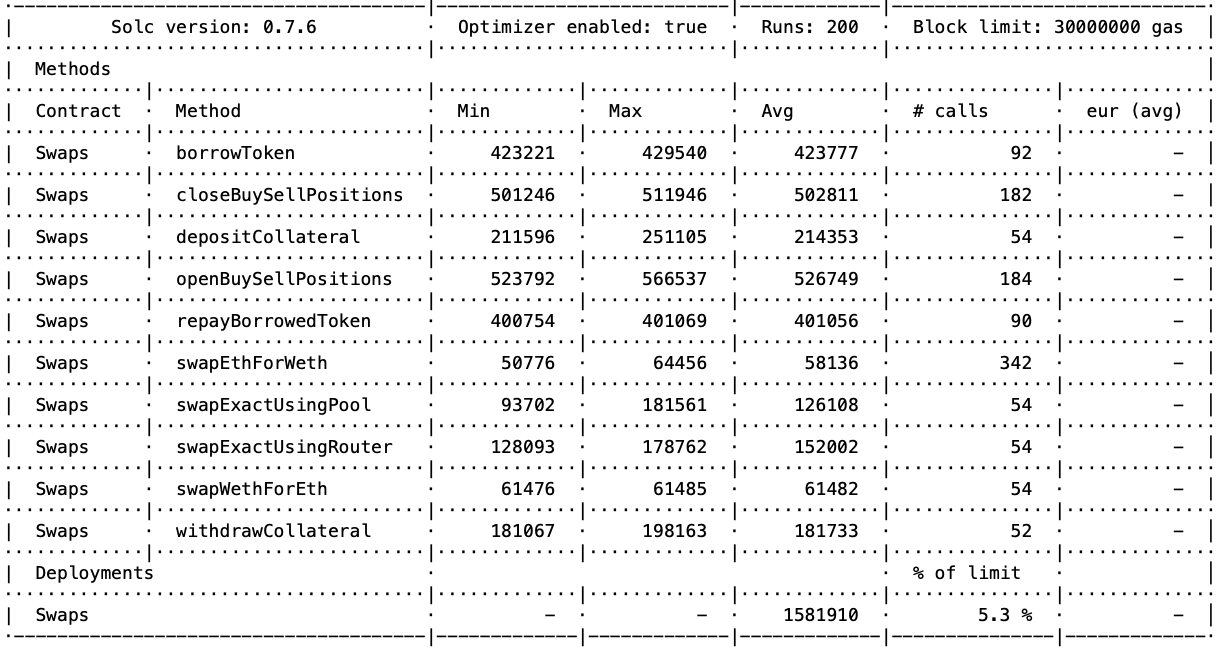
\includegraphics[width=0.9\textwidth]{project/Images/gas_fee_results.png}
    \caption{Results from running smart contract functions \label{fig:gasResult}}
\end{figure}

\begin{figure}[htb!]
    \centering
    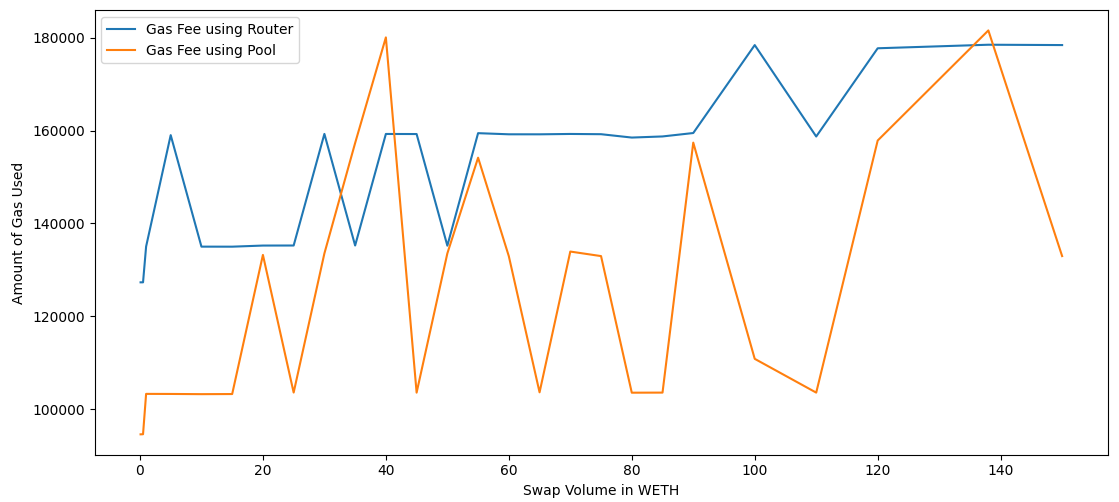
\includegraphics[width=0.75\textwidth]{project/Images/SwapFeesPlot.png}\\
    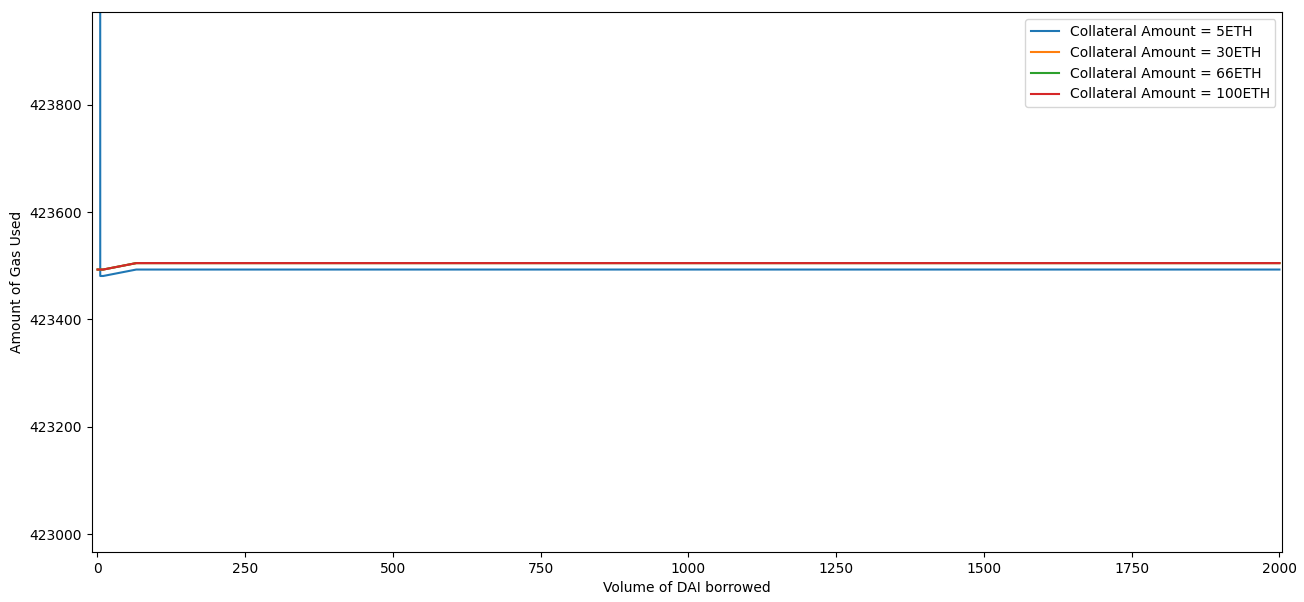
\includegraphics[width=0.75\textwidth]{project/Images/BorrowFees2.png}
    \caption{Gas Usage Plots of Gas Used by Swapping (Top) and Borrowing (Bottom) \label{fig:gasPlots1}}
\end{figure}

\begin{figure}[htb!]
    \centering
    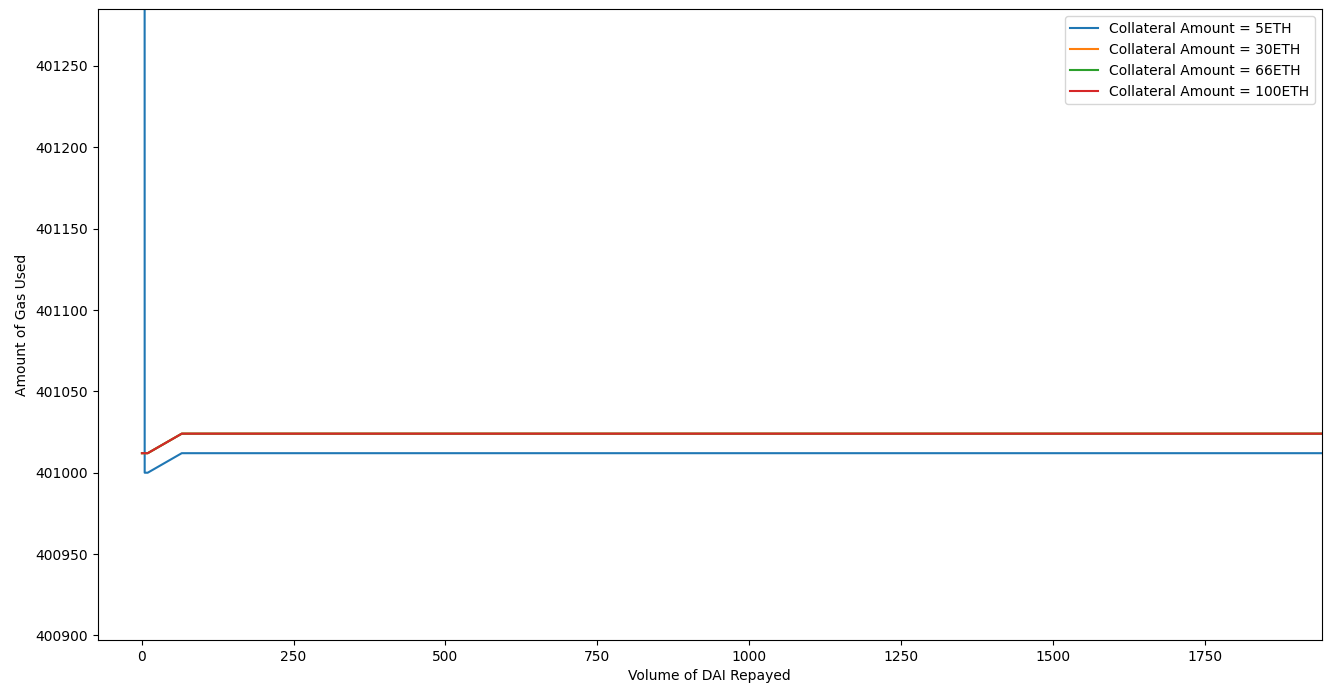
\includegraphics[width=0.75\textwidth]{project/Images/RepayFees2.png}\\
    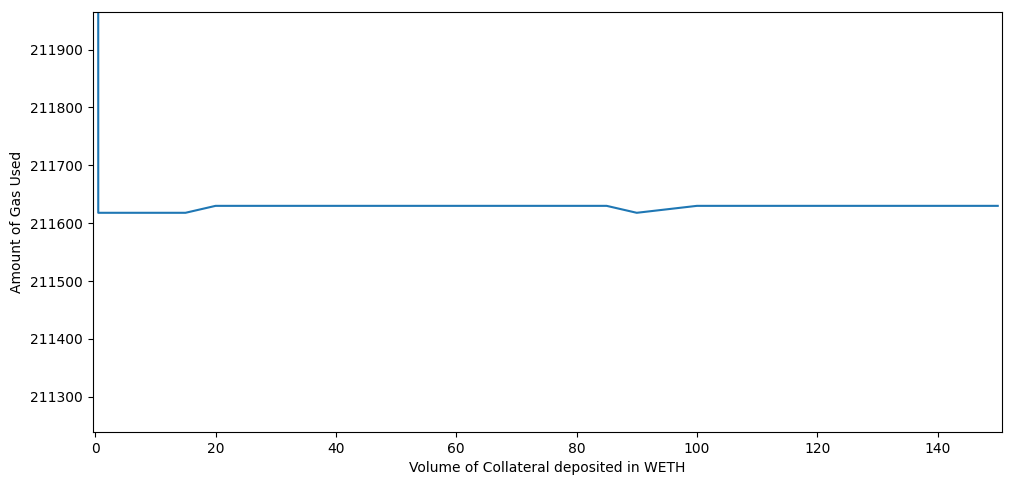
\includegraphics[width=0.75\textwidth]{project/Images/depositFeesPlot2.png}
    \caption{Gas Usage Plots of Gas Used by Repaying Borrowed Tokens (Top) and Depositing additional tokens (Bottom) \label{fig:gasPlots2}}
\end{figure}

\noindent Upon analysing these plots, it becomes apparent that the majority of the functions exhibit a high level of consistency. However, it is noteworthy that for the smallest quantity tested, the gas consumption is significantly higher than that of larger quantities. Nevertheless, once this threshold is surpassed, gas usage remains consistent. Therefore the average gas usage of each operation is used in the backtesting system as it provides a representative estimate of the gas consumption across different quantities.
\\[3mm]
Furthermore, another interesting feature is the gas usage by swaps and the different methods. The initial method utilises Uniswap's Router, which scans all available liquidity pools to identify the optimal price, whereas the second method involves direct swapping within a specific liquidity pool. Figure \ref{fig:gasPlots1} illustrates that, on average, the router-based approach exhibits higher gas usage than direct swapping using a liquidity pool. However, directly swapping using a liquidity pool exhibits greater volatility in gas consumption but also consistently returns to values above 100,000; because of this, the average gas usage of swapping using a liquidity pool is used.
\\[3mm]
It can also be seen that combining the operations to open/close buy and sell positions consumes less gas compared to if they were to be executed separately. This also confirms the claims in Wang's paper that batching the operations together is more effective than executing them separately~\cite {wang_cyclic_2022}. Thus incorporating this into the backtesting system, each order deducts some ETH, which is calculated by how much gas is used by the order type multiplied by the gas price. For example, in the case of buying more ETH:
\begin{lstlisting}[language=Python]
amount_to_swap = self.account['WETH'] * order[1]
self.account['WETH'] = self.account['WETH'] - amount_to_swap
self.account['ETH'] = self.account['ETH'] + amount_to_swap - (GAS_USED_BY_BUYING_ETH * gas_price_in_eth)
\end{lstlisting}
\vspace{5mm}
\noindent However, in order to analyse the impact of combining operations on strategy returns, the deduction of ETH for gas fees for both \texttt{OPEN} and \texttt{CLOSE} orders is handled differently. Instead of deducting the fees immediately upon each order, the deduction is performed after iterating through the trading signal. If the signal contains such orders, the necessary amount of gas fee is deducted based on whether the orders are specified, by the parameter \texttt{should\_batch\_trade}, to be batched or executed separately. The code for handling this can be seen in Appendix \ref{app:deducting-gas-fee}.

\subsection{Validating Balance Health}
To maintain the integrity and effectiveness of the trading strategy, it is crucial to incorporate various checks and safeguards after each trade and at each timestep. One key aspect involves monitoring the balance of each token to ensure that it remains positive. After every order execution, the tokens' balances are checked, and if any of them fall below zero, an exception is triggered.
\begin{lstlisting}[language=Python]
if self.account['T1'] < negative_threshold:
    raise Exception('Account balace goes below 0 - T1')
if self.account['T2'] < negative_threshold:
    raise Exception('Account balace goes below 0 - T2')
if self.account['WETH'] < negative_threshold:
    raise Exception('Account balace goes below 0 - WETH')
if self.account['ETH'] < negative_threshold:
    raise Exception('Account balace goes below 0 - ETH')
\end{lstlisting}
Furthermore, the loan-to-value ratio is calculated to simulate the potential liquidation of a sell position's loan. This ratio serves as an indicator of the position's health and risk level. If the loan-to-value ratio breaches the predefined liquidation threshold, an exception is thrown, indicating that the position is approaching an unsustainable state.
\begin{lstlisting}[language=Python]
sell_token, sold_price, sell_volume, _ = sell_trade
current_token_price = prices[f'P{sell_token[1]}']
curr_value_of_loan_pct = (sell_volume * current_token_price) / self.account['collateral_WETH']
if round(curr_value_of_loan_pct, 4) > liquidation_threshold:
    raise Exception(f'Short position liquidated')
\end{lstlisting}

\section{Live Trading}
A similar approach is required to run the strategies live; however, the execution system and balance tracking are altered. For the system, multiple components are required for live trading to occur. The first is the ability to interact with the blockchain to execute the orders; handled by smart contracts; the second is to manage the state of the strategy, accounts and open positions for the strategies to use to generate signals, and finally, a method to convert the signal into smart contract invocations to execute the orders—the workflow of trading on the live execution system.
\begin{figure}[H]
    \centering
    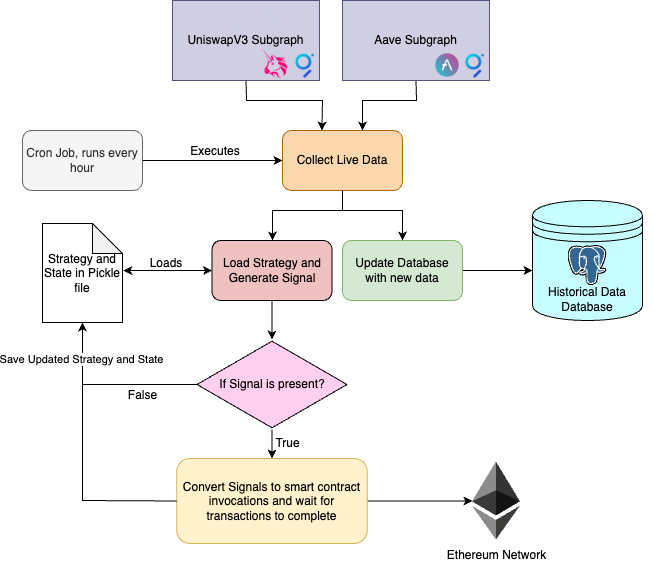
\includegraphics[width=0.99\textwidth]{project/Images/live-trading-system-diagram.png}
    \caption{Flowchart of trading a strategy live \label{fig:live-flow}}
\end{figure}

\subsection{Smart Contracts}
\label{sec:smart-contracts}
In order to be able to interact with Uniswap and Aave over Ethereum, smart contracts are written, which are then deployed on the blockchain network. Functions that the smart contract possesses can then be executed by anyone who knows the contract's address on the network. Smart contracts are programmable protocols written in Solidity, a high-level programming language designed for creating and executing smart contracts on Ethereum. For trading using the mentioned strategies, a few the following functionalities are required to be implemented; wrapping ETH for WETH, unwrapping WETH, swapping token A for token B using a given liquidity pool and finally, borrowing and repaying some of token A using WETH as collateral. The first two functions are required if the trader has only ETH in their account; thus, by wrapping the ETH, they can trade ETH as an ERC-20 token. ERC-20 is a widely adopted technical standard to create interchangeable Ethereum blockchain tokens. It provides developers with the framework to design tokens compatible with various applications and services operating within the Ethereum ecosystem. These tokens are designed to represent a variety of assets, most importantly cryptocurrencies.

\subsubsection{Wrapping of ETH and Unwrapping WETH}
This functionality is required if the trader has only ETH in their account; thus, by wrapping the ETH, they could trade ETH in its ERC-20 format, WETH. The functions of wrapping ETH and unwrapping WETH can be seen in Figure \ref{fig:sol-code-eth-weth}, where \texttt{swapEthForWeth} wraps ETH and \texttt{swapWethForEth} unwraps WETH. The \texttt{swapEthForWeth} function first uses the \texttt{IWETH} interface, which is itself an ERC20 interface, to allow functions such as transfer of ownership of the token, to deposit an amount of ETH in exchange for WETH, which is then transferred back to the address of the caller. The \texttt{swapWethForEth} function unwraps the WETH by first sending the specified volume of WETH from the caller to the smart contract, withdrawing the specified amount from the IERC20, which calls the \texttt{receive} function to enable the receiving of ETH and once the ETH is withdrawn into the smart contract's account, it is transferred back to the caller.

\begin{figure}[htb!]
\begin{adjustwidth}{-0.5in}{-0.5in}
\begin{minipage}{\linewidth}
\centering
\begin{lstlisting}[language=Solidity]
interface IWETH is IERC20 {
  function deposit() external payable;
  function withdraw(uint amount) external;
}

address public immutable wethAddress = 0xC02aaA39b223FE8D0A0e5C4F27eAD9083C756Cc2;

function swapEthForWeth() external payable {
    IWETH weth = IWETH(wethAddress);
    weth.deposit{ value: msg.value }();
    weth.transfer(msg.sender, msg.value);
}

function swapWethForEth(uint256 amount) external payable {
    IWETH(wethAddress).transferFrom(msg.sender, address(this), amount);
    IWETH(wethAddress).withdraw(amount);
    msg.sender.transfer(address(this).balance);
}

receive() external payable {}
\end{lstlisting}
\end{minipage}
\end{adjustwidth}
\caption{Solidity Code for Interchanging between ETH and WETH \label{fig:sol-code-eth-weth}}
\end{figure}

\subsubsection{Swapping using a Uniswap Liquidity Pool}
Swapping using a Uniswap liquidity pool is also another critical functionality. This is done by using the \texttt{IUniswapV3Pool} interface to expose the liquidity pool's functions and calling swap on it using the necessary parameters. The parameters, in their respective order, are the address of the recipient of the swapped tokens, a boolean on whether the swap direction is from token0 to token1 or vice versa, the volume of the source token that would like to be swapped, an integer (sqrtPriceLimitX96) that manages how much slippage is acceptable, and finally the ABI encoded data that is required in the callback function. When calling \texttt{swap} function, the sqrtPriceLimitX96 parameter is set to ignore the effects of slippage and proceed with the swap. Finally, once the swap has taken place, Uniswap calls the callback function \texttt{uniswapV3SwapCallback}, with transfers the swapped tokens to the caller of the function. See Figure \ref{fig:sol-code-swap}.

\begin{figure}[htb!]
\begin{adjustwidth}{-0.5in}{-0.5in}
\begin{minipage}{\linewidth}
\centering
\begin{lstlisting}[language=Solidity]
function swapExactUsingPool(address poolAddress, bool zeroForOne, int256 amountIn) public returns (int256, int256) {
    IUniswapV3Pool pool = IUniswapV3Pool(poolAddress);
    return
        pool.swap(msg.sender, zeroForOne, amountIn, zeroForOne ? TickMath.MIN_SQRT_RATIO + 1 : TickMath.MAX_SQRT_RATIO - 1, abi.encode(poolAddress, pool.token0(), pool.token1(), msg.sender));
}

function uniswapV3SwapCallback(int256 amount0Delta, int256 amount1Delta, bytes calldata data) external override {
    (address poolAddress, address token0, address token1, address userAddress) = abi.decode(data, (address, address, address, address));
    require(msg.sender == address(poolAddress));
    if (amount0Delta > 0) {
        IERC20(token0).transferFrom(
            userAddress,
            msg.sender,
            uint256(amount0Delta)
        );
    }
    if (amount1Delta > 0) {
        IERC20(token1).transferFrom(
            userAddress,
            msg.sender,
            uint256(amount1Delta)
        );
    }
}
\end{lstlisting}
\end{minipage}
\end{adjustwidth}
\caption{Solidity Code for Swapping using Uniswap \label{fig:sol-code-swap}}
\end{figure}

\subsubsection{Borrowing and Repaying Tokens using Aave}
To allow for short selling, borrowing and repaying tokens are required; therefore, interacting with Aave in the smart contract is essential. The first step is to instantiate the lending pool using Aave's \texttt{PoolAddressesProvider}. When borrowing, some collateral is set aside to be able to borrow any number of tokens; thus, the first step is to deposit this collateral into the lending pool and allow it to be used as collateral (Lines 1-8). Secondly, the specified token is borrowed from the lending pool using the variable interest rate specified by the third argument in the \texttt{borrow} function; once received, the tokens are sent to the caller's address. The opposite methodology is true for loan repayment; the tokens are transferred from the caller's address to the smart contract's address, which is then sent back to the lending pool by the \texttt{repay} function. The collateral is withdrawn and automatically sent to the caller's address. See Figure \ref{fig:sol-code-aave}.

\begin{figure}[htb!]
\begin{adjustwidth}{-0.5in}{-0.5in}
\begin{minipage}{\linewidth}
\centering
\begin{lstlisting}[language=Solidity]
IPool public immutable lendingPool = IPool(IPoolAddressesProvider(0x2f39d218133AFaB8F2B819B1066c7E434Ad94E9e).getPool());

function borrowToken(address tokenAddress, uint256 borrowAmount, uint256 collatoralAmount) public {
    // Deposit Collatoral
    IERC20(wethAddress).transferFrom(msg.sender, address(this), collatoralAmount);
    IERC20(wethAddress).approve(address(lendingPool), collatoralAmount);
    lendingPool.deposit(wethAddress, collatoralAmount, address(this), 0);
    lendingPool.setUserUseReserveAsCollateral(wethAddress, true);

    // Borrow token
    lendingPool.borrow(tokenAddress, borrowAmount, 2, 0, address(this));
    IERC20(tokenAddress).transferFrom(address(this), msg.sender, borrowAmount);
}

function repayBorrowedToken(address tokenAddress, uint256 repayAmount, uint256 collateralWithdrawAmount) public {
    IERC20(tokenAddress).transferFrom(msg.sender, address(this), repayAmount);
    IERC20(tokenAddress).approve(address(lendingPool), repayAmount);
    lendingPool.repay(tokenAddress, repayAmount, 2, address(this));
    lendingPool.withdraw(wethAddress, collateralWithdrawAmount, msg.sender);
}
\end{lstlisting}
\end{minipage}
\end{adjustwidth}
\caption{Solidity Code for Borrowing and Paying on Aave \label{fig:sol-code-aave}}
\end{figure}
\subsubsection{Opening and Closing of Trading Positions}
In addition to these functions, it is known that batching transactions together is more efficient than having to execute them separately, therefore as the strategies being explored for this project require both a buying and selling trade each time, the functions \texttt{openBuySellPositions} and \texttt{closeBuySellPositions} have been implemented such that it follows the method mentioned in Subsection \ref{sec:buying-selling}, combining the internal functions \texttt{swapExactUsingPool}, \texttt{borrowToken} and \texttt{repayBorrowedToken}. The full implementation can be found in Appendix \ref{fig:sol-code-open-close}.

\subsection{State}
Storing the state of the strategy is essential as the strategies need to store and maintain its history and variables to ensure consistency when trading; therefore, the state is stored as a dictionary in a pickle file. The state contains the liquidity pool pair being traded, the strategy instance, a dictionary of the open positions (initially empty) and the account balance. The state is updated after every execution and stored in the pickle file.

\subsection{Retreival of Data and Signal Generation}
The frequency at which signals and data are collected is easily variable; however, the current design has a frequency of every hour to ensure consistency. This frequency is set in a Cron job. The Cron job runs a script to collect the current price data and generate a signal. Using Uniswap's subgraph, two queries are sent to retrieve the necessary data. The first query queries the liquidity pool returning its current prices, and the second, retrieves the most recent transaction, regardless of the type of transaction, to collect the cost of gas at the time. These data points are inserted into their corresponding tables in the database. They are also sent to the strategy to generate a signal, which is sent to the execution system for execution. The GraphQL queries are in Appendix \ref{app:live-pool-price-query} and \ref{app:live-gas-query}.

\subsection{Trade Execution}
Once the signal has been received, it is sent to the trade execution system. Once the signal is required to be actualized, the execution system breaks the signal into different types of orders and executes them. For each type of order in signal, its parameters are extracted, e.g. volume to buy, volume to sell, the target token and the prices when opening a position. These parameters are then used to calculate the remaining parameters required to call the corresponding smart contract function, e.g. the swap direction's zeroForOne. Finally, once all the necessary function parameters have been defined, the order is executed on the blockchain by performing four steps. The first is calling the smart contract function, signing the transaction, sending the transaction and waiting for the transaction to complete. After all of the orders have been executed, the new balances of each token along with the updated \texttt{open\_positions} is returned to then be stored as the new state.
\begin{figure}[htb!]
\begin{adjustwidth}{-0.5in}{-0.5in}
\begin{minipage}{\linewidth}
\centering
\begin{lstlisting}[language=Python]
# Call the order's corresponding function
call_function = contract.functions.<Smart Contract Function Name>(<Function Paramters>).buildTransaction({"chainId": Chain_id, "from": caller, "nonce": nonce})
# Sign transaction
signed_tx = web3.eth.account.sign_transaction(call_function, private_key=private_key)
# Send transaction
send_tx = web3.eth.send_raw_transaction(signed_tx.rawTransaction)
# Wait for transaction receipt
tx_receipt = web3.eth.wait_for_transaction_receipt(send_tx)
\end{lstlisting}
\end{minipage}
\end{adjustwidth}
\end{figure}
